In this section, We present the the I/O performance of our plugin. These experiments are not targeted towards performing a semantic analysis of data, such as active analysis or semantic restructuring discussed in the previous section.
For evaluation purposes, we have used HDF5's \textit{h5perf} performance tool~\cite{h5perf}. It allows configuring various parameters, such as the number of processes, number of datasets, amount of data read/written by a process in a single I/O call (transfer size) etc. For our measurements, we created 10 1-dimensional datasets, and the total file size was 64 GB or more.
In every run, every process contributed equal amount of data per dataset using the default individual (non-collective) I/O mode of h5perf.

Tests were performed on the Lustre parallel file system~\cite{lustre} on the Atlas cluster at University of Dresden. The file system has 12 OSTs with a stripe size of 1MB. The file system is connected to the compute nodes using an SDR Infiniband link. The cluster has 92 AMD Opteron nodes with 64 cores each and 64 to 512 GB memory. Tests were run thrice and we present the average bandwidth values, which does not include the time taken to open and close the file.

We have performed tests with 1,2,4,8,32 and 64 processes with a maximum of 4 processes per node.
Reads and writes are either contiguous or interleaved; processes either access contiguous locations in file or execute a strided pattern.
We compare the performance of the default MPI-IO driver, our plugin, and the PLFS MPI-IO driver (ad\_plfs). 

In Figure~\ref{write_contig}, we show the write performance for a transfer size of 1MB for contiguous writes. It can be seen that the plugin regularly outperforms MPI-IO except for the 64 process case, where the metadata overhead incurred by the plugin is high. The performance  of ad\_plfs is the best for higher process counts. Figure~\ref{read_contig} shows the performance of contiguous reads. 
%Figure~\ref{write_interleaved} shows the performance of unaligned writes for a maximum of 8 processes. We set the transfer size here to be 10 bytes more than 1MB. Also, the writes here are interleaved as opposed to contiguous. We see a similar pattern, where the plugin outperforms MPI-IO, but is not as good as that of ad\_plfs for 8 processes. 
Figures~\ref{write_interleaved} and~\ref{read_interleaved} show the interleaved write and read performance respectively for an unaligned transfer size (1M + 10bytes) for a maximum of 8 processes. The write performance of MPI-IO is quite poor in this case. The plugin easily outperforms MPI-IO and almost matches the performance of ad\_plfs. 

Overall, results show that the plugin consistently shows good performance, however it does not scale as well as ad\_plfs. This is due to the fact that since we are directly making calls to the PLFS API, the metadata overhead is high. All processes participate in file open and close operations, which for large problem sizes adds significant overhead. Hence, for future work, we plan to use ad\_plfs directly in the plugin which can overcome this performance drawback, since ad\_plfs has collective optimizations in open and close. It should be noted that there are some MPI libraries tailored to suit specific types of applications and which do not provide an implementation for MPI-IO. Such libraries can benefit from using a plugin that does not rely on MPI-IO. 

\begin{figure}[!t]
\centering
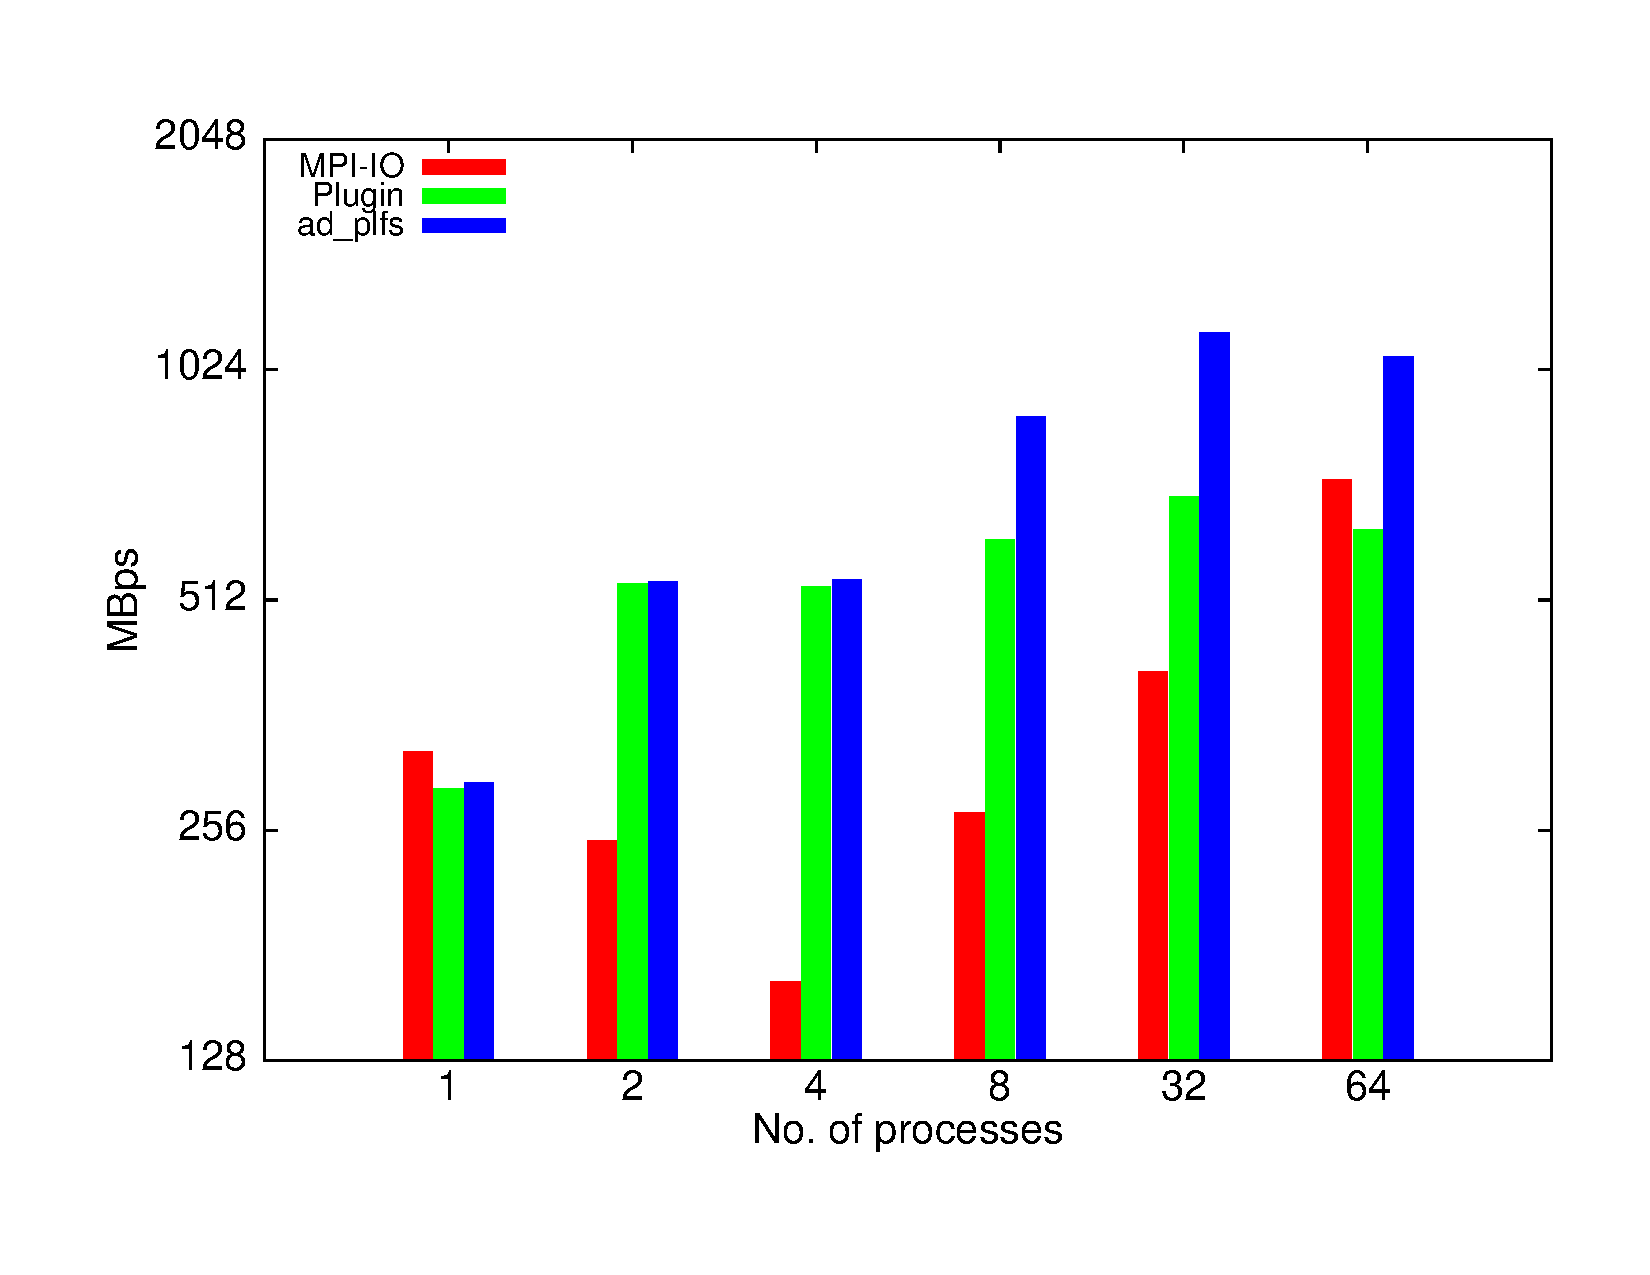
\includegraphics[width=3.6in,height=3.0in]{contig_w}
\caption{Performance of contiguous writes}
\label{write_contig}
\end{figure}

\begin{figure}[!t]
\centering
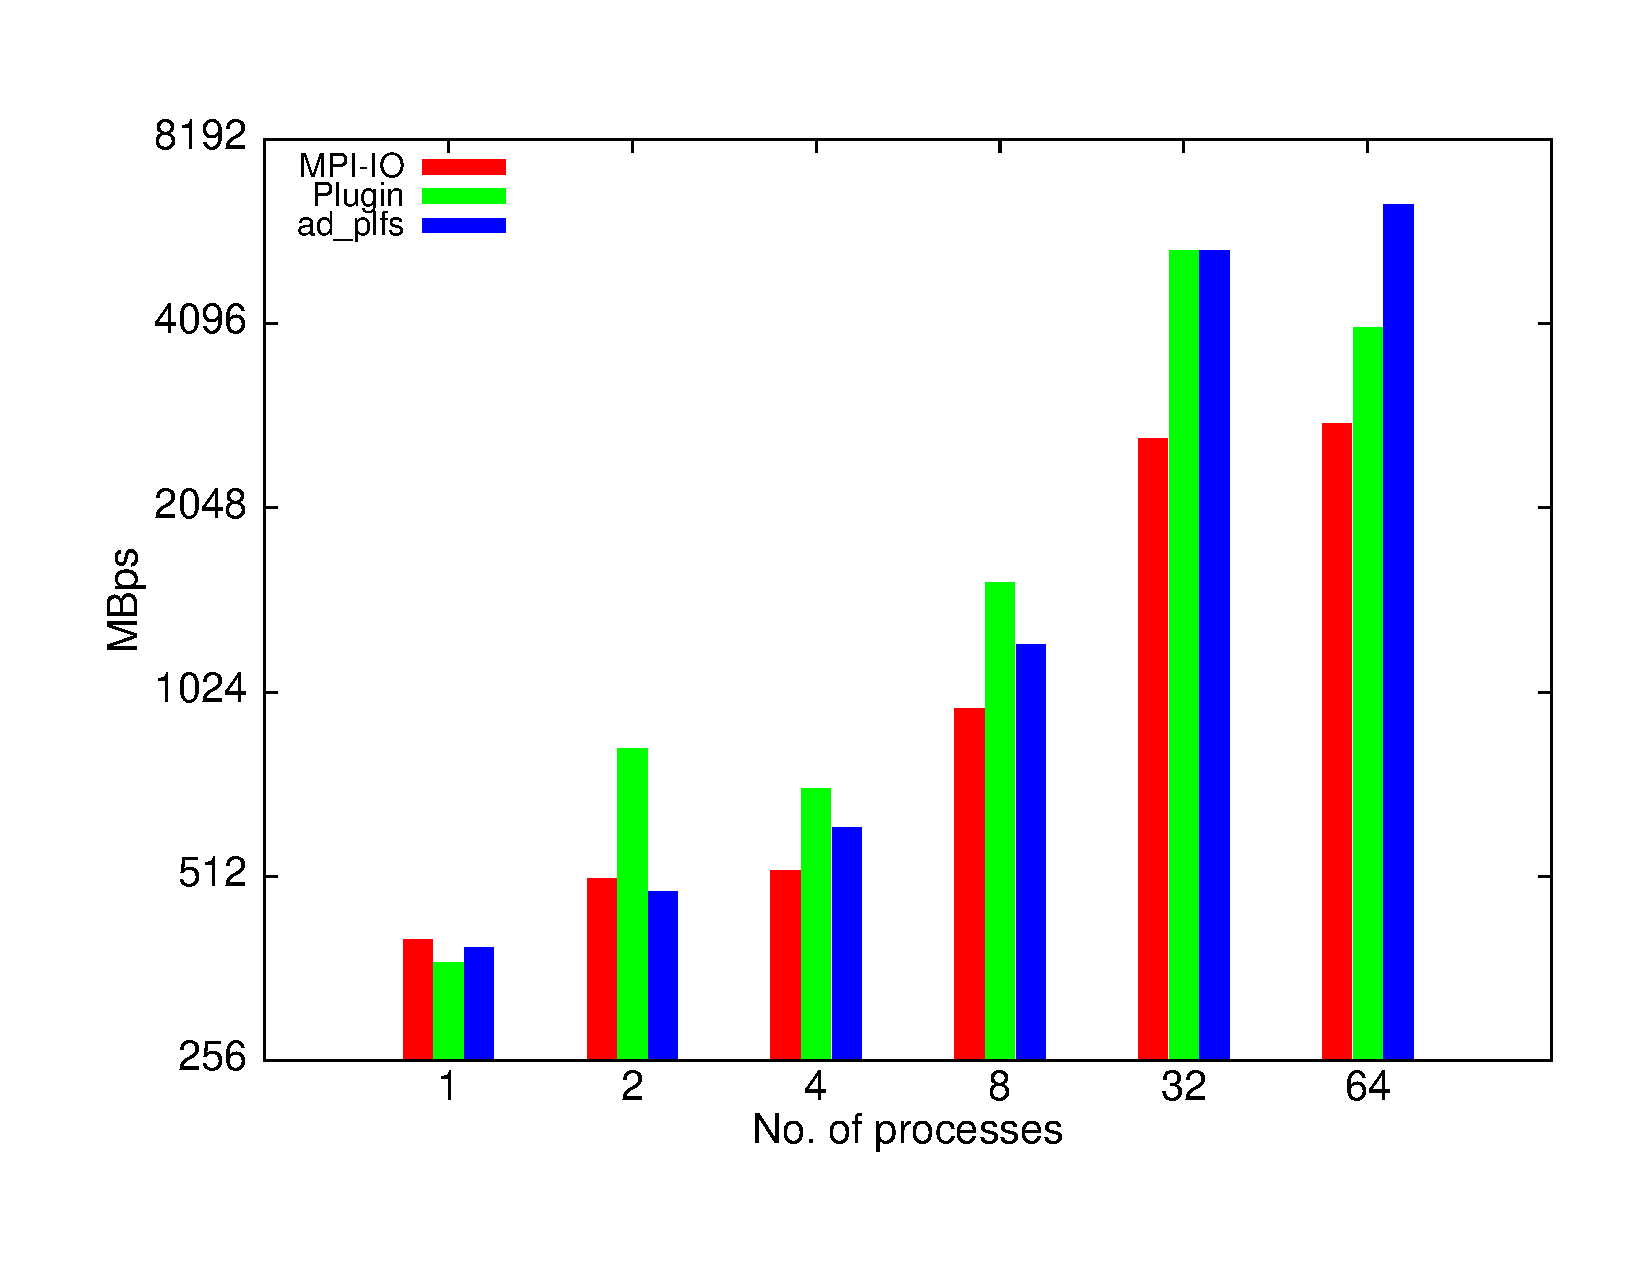
\includegraphics[width=3.6in,height=3.0in]{contig_r}
\caption{Performance of contiguous reads}
\label{read_contig}
\end{figure}

\begin{figure}[!t]
\centering
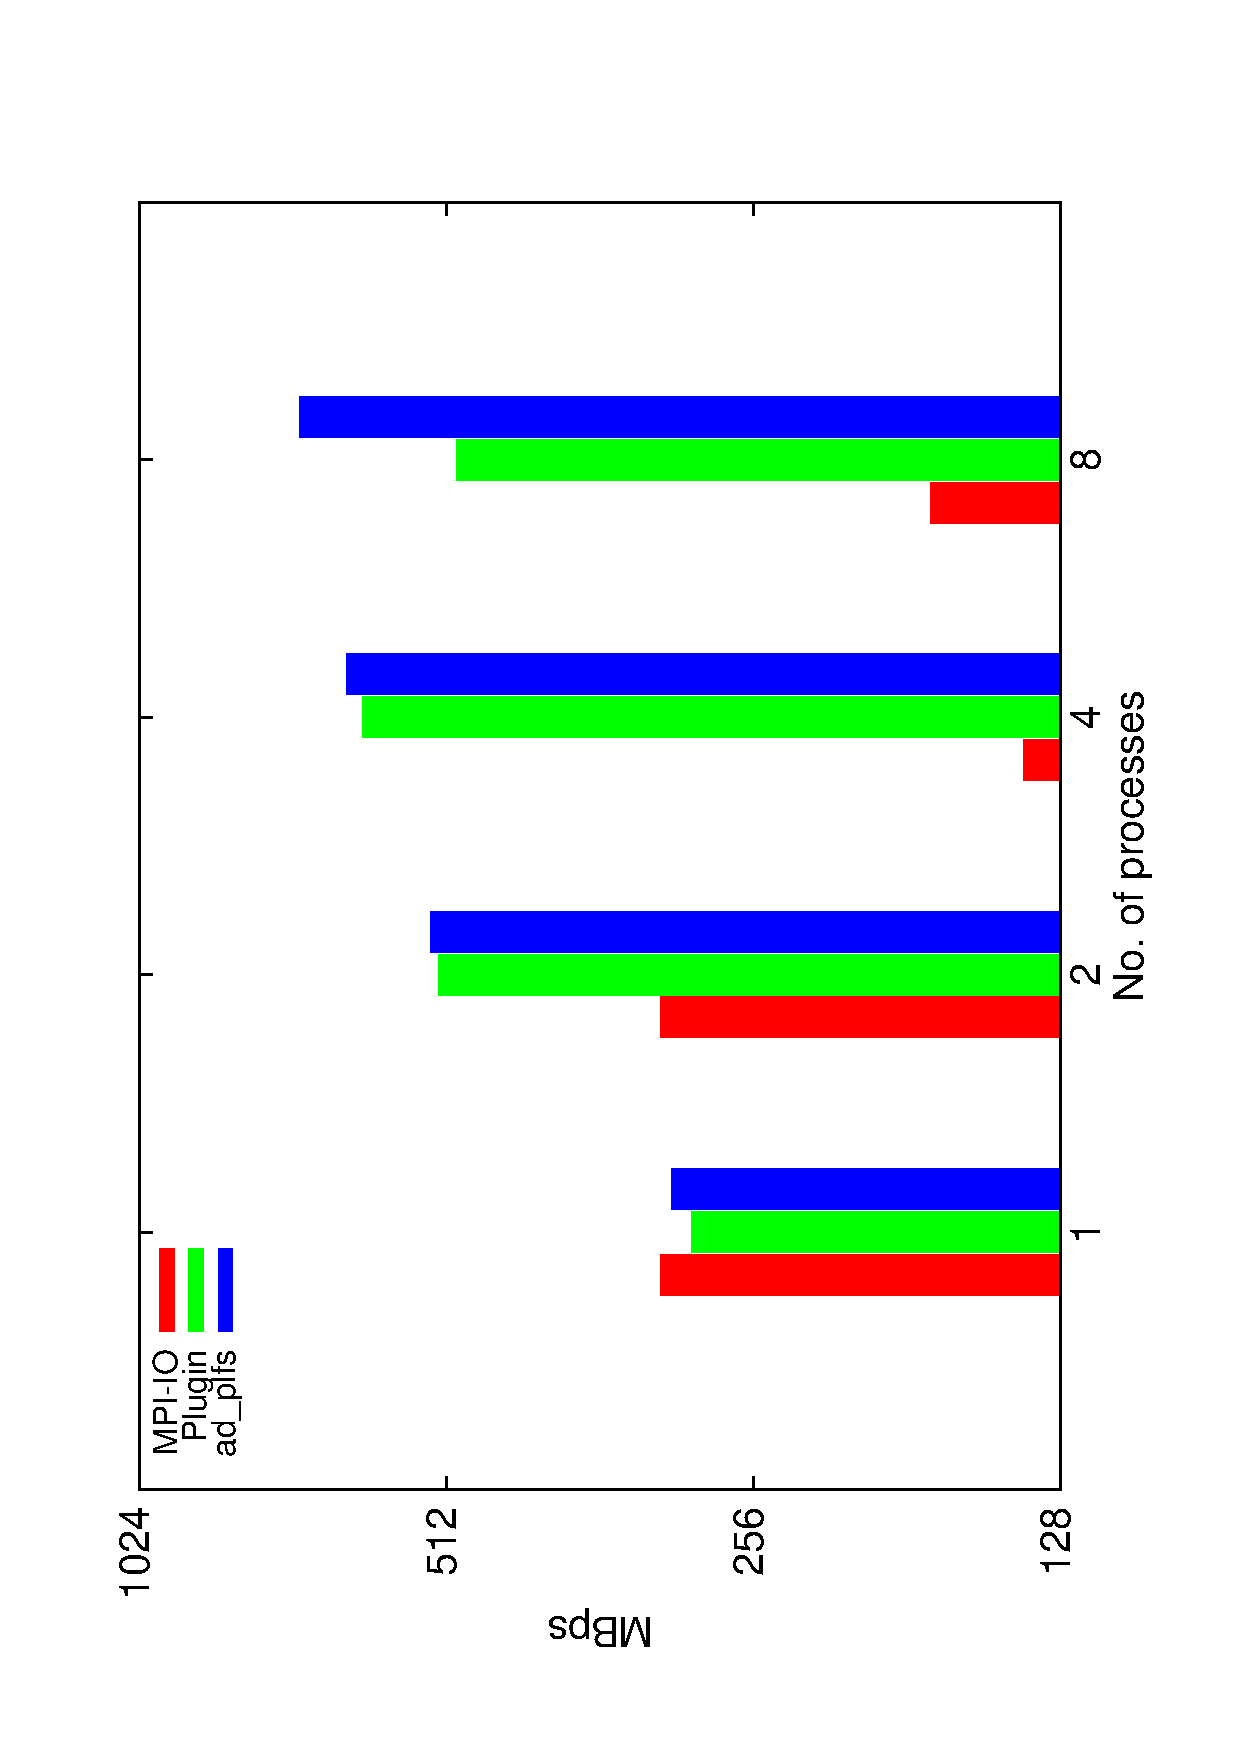
\includegraphics[width=3.6in,height=3.0in]{interleaved_w}
\caption{Performance of interleaved, unaligned writes}
\label{write_interleaved}
\end{figure}

\begin{figure}[!t]
\centering
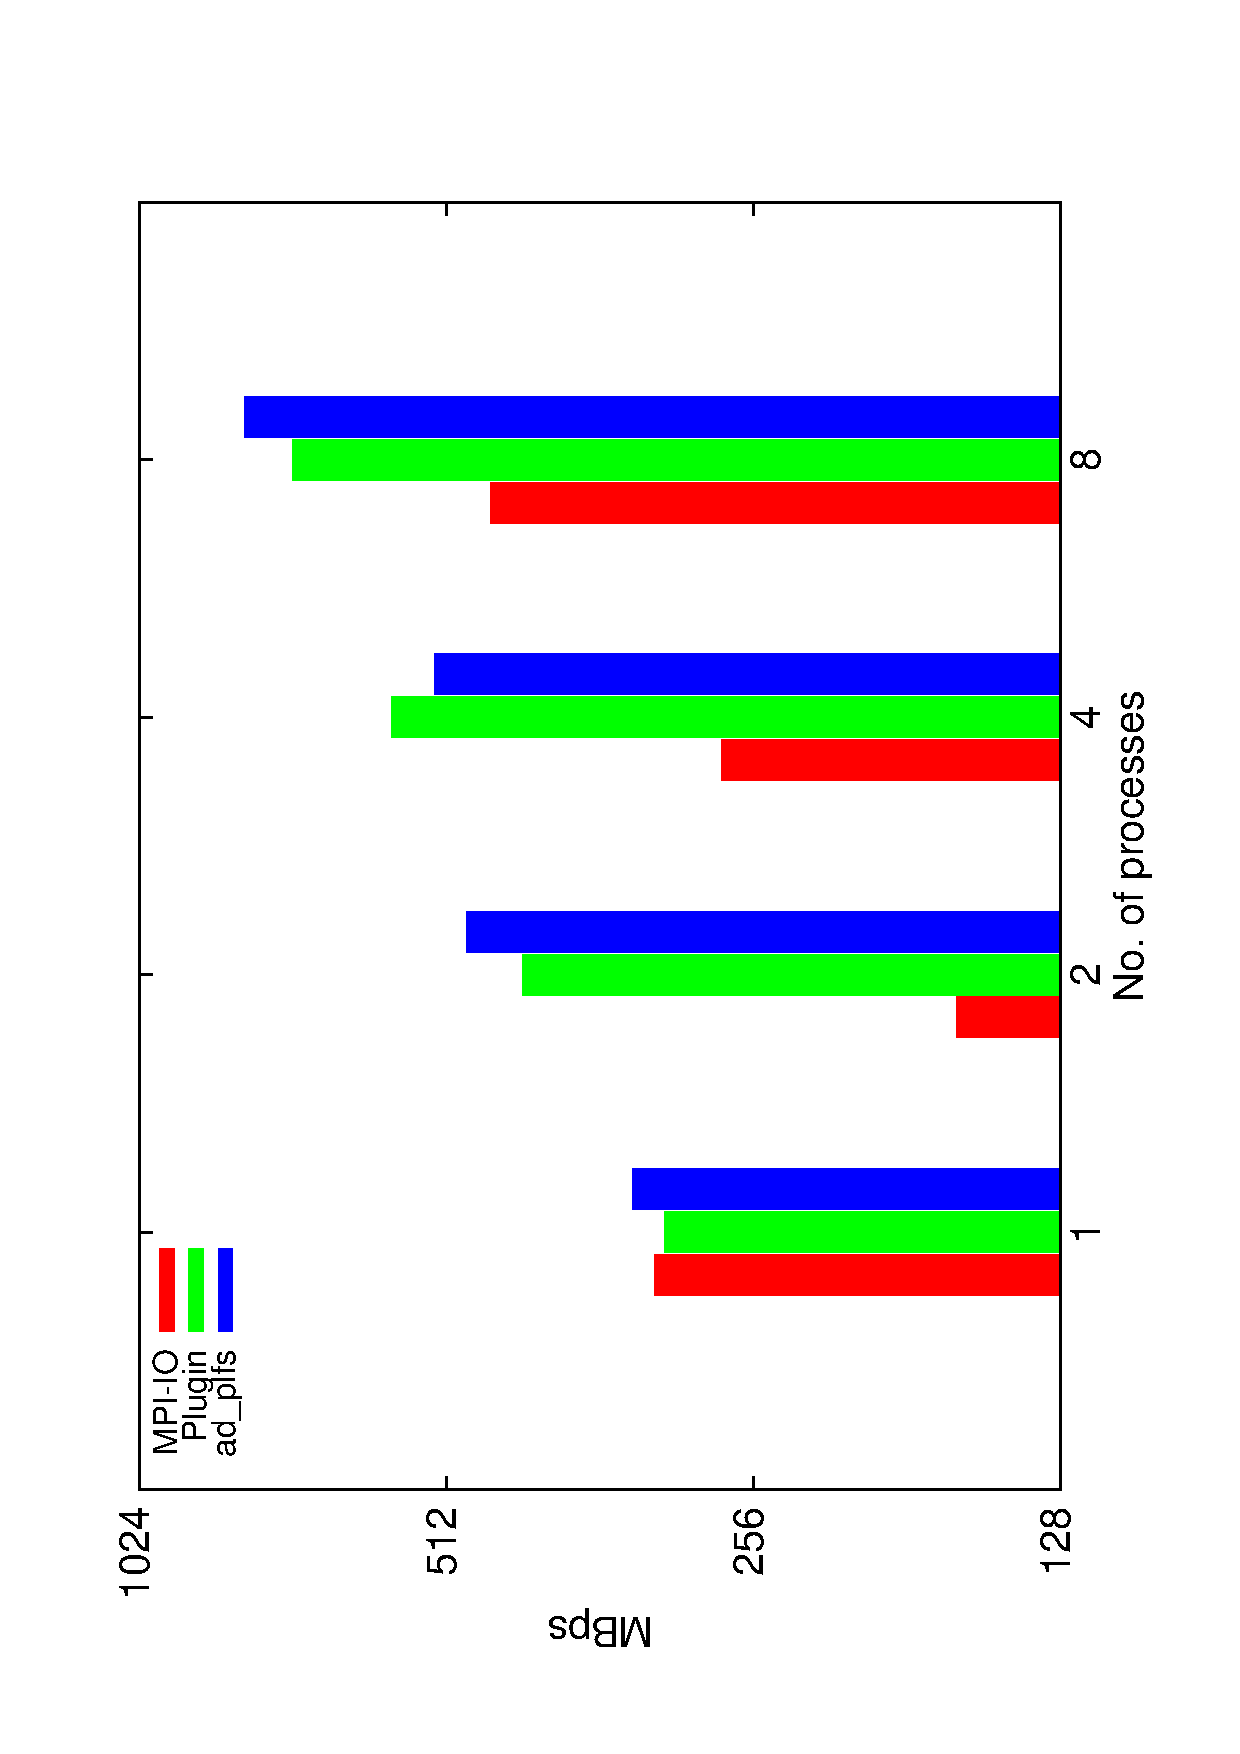
\includegraphics[width=3.6in,height=3.0in]{interleaved_r}
\caption{Performance of interleaved,unaligned reads}
\label{read_interleaved}
\end{figure}


